\newpage
\activity\section{Adders and Destiny (Density!)}

\begin{prob} 
Contrary Clark states that he knows a simpler method of adding
fractions. He views $1/3$ as ``$1$ of $3$'' and $3/4$ as ``$3$ of
$4$.''
\[
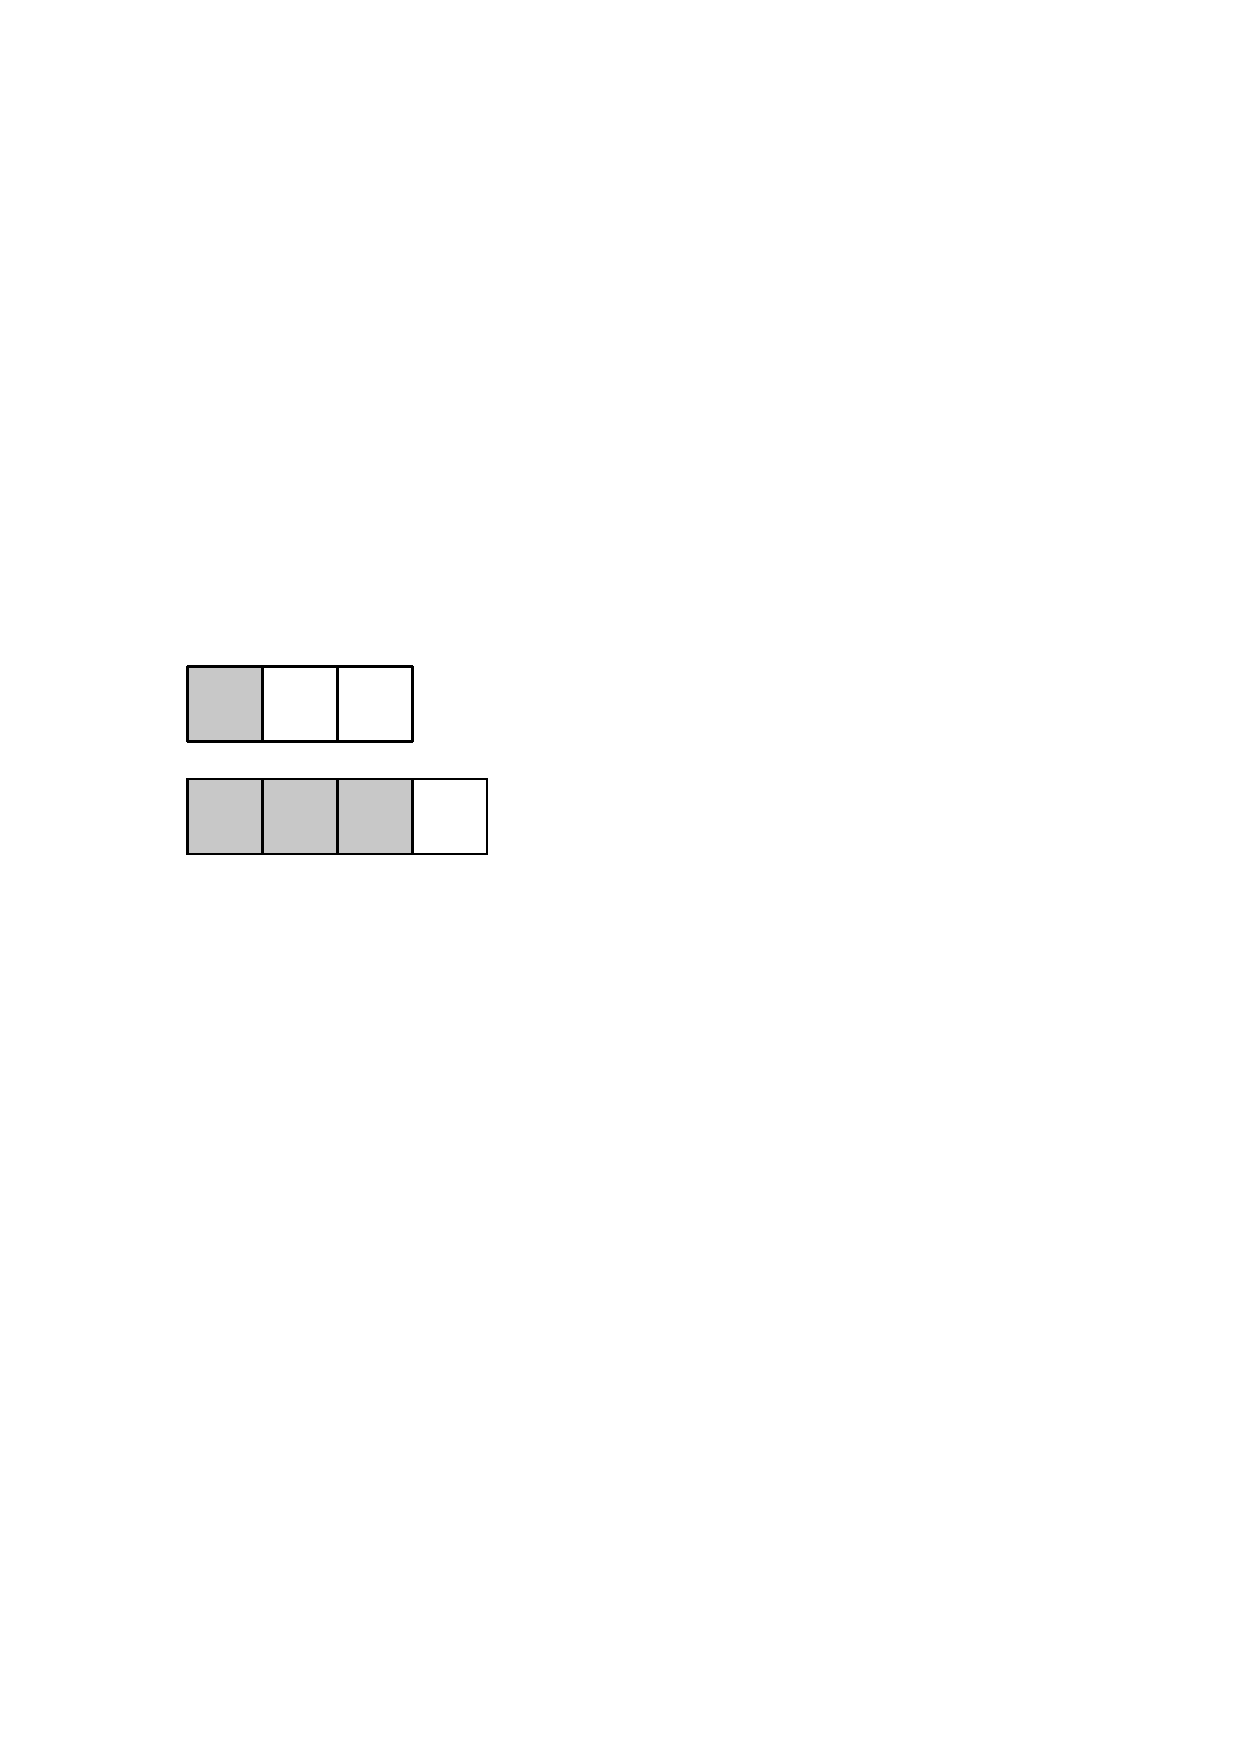
\includegraphics{../graphics/clark.pdf}
\]
From this viewpoint Contrary Clark claims:
\[
\frac{1}{3} + \frac{3}{4} = \frac{4}{7}
\]
How do we set Contrary Clark straight?
\end{prob}


Sometimes in mathematics, we go a little crazy---in a good way. Let me
explain: Can we find value in Contrary Clark's erroneous method of
``adding'' fractions? Before we can answer this question, we must gain
a deeper understanding of the method.

\begin{prob}
 Draw a number line, plot the points
\[
\frac{1}{3}, \qquad \frac{3}{4}, \qquad\frac{1+3}{3+4}, \qquad\frac{1}{3} + \frac{3}{4}.
\]
What do you observe? Play around with other numbers. Can you explain
why the operation of ``adding the numerators'' and ``adding the
denominators'' is sometimes called the \textit{mediant}\index{mediant}
of two fractions?
\end{prob}


\begin{prob} 
I'm thinking of a number. Explain how to use the mediant to find other
numbers that are arbitrarily close to my number.
\end{prob}


\begin{prob} In light of our discussion above, compare/contrast the two story problems below:
\begin{enumerate}
\item Bart has been shooting free-throws. On Monday he made 18 out of 101. On Tuesday he made 18 out of 121. On Wednesday he made 17 out of 120. What is his average for the 3 days?
\item Vic has been eating chocolate. On Monday he ate $1/3$rd of a candy bar. On Tuesday he ate $3/5$ths of a candy bar. On Wednesday he ate $1/4$th of a candy bar. How much chocolate did Vic eat over the three days?
\end{enumerate}
\end{prob}
